\documentclass[../Matt_Gebert_Honours_Thesis.tex]{subfiles}

\begin{document}
	
%	I will then describe the devices and measurements I have made in \cref{chap:fab&characterisation}. This will regard connections to devices, which allow the measurements I have perform, and the processes used to fabricate our devices. I have made graphene devices using lithography and evaporation methods, to create electrical contacts. I will also describe the oxides I have investigated in this chapter, and the methods I have used to transfer them.

	To create devices where we can measure the electronic properties referenced in \cref{sec:fet,sec:electronic_properties}, metalic contacts need to be added to the graphene to measure electronic flow through the device. 
	
	To do this, lithography can be used to create polymer structures that allow the deposition of desired material in 2D geometries. This process and the adjustements made for fabricating our devices are described in the sections below.

	\section{Lithography}\label{sec:lithography}
		Lithography typically consists of three steps.
		\begin{enumerate}
			\item Spin coating - covering your sample with a uniform layer of polymer.
			\item Exposure - exposing the polymer to light changes the chemical compounds and properties. This differentiates exposed areas to those unexposed.
			\item Developer solution - developer solution removes indended areas of photoresist to create structures.
		\end{enumerate}
		
	\subsection{Spin coating photoresists}\label{sec:resists}
		A spin coater is used to deposit thin films of materials. A vacuum is used to hold a sample horizontally on the spinner, before drops of photoresist are dropped onto the sample. The sample is then spun over sometime to achieve a uniform thickness of the photoresist, before baking on a hotplate occurs to set the sample.
		
		Photoresists vary in their spinning thickness, but also their exposure rates. Positive photoresists dissolve in developer when exposed to light, while negative photoresists dissolve if not exposed to light. We have only used positive photoresists, as we have primarily been creating structures for deposition, and not etching material (protect your sample, but remove everything else).
		
	\subsubsection{HMDS \& AZ-1512HS}
		Initially devices were fabricated using the AZ-1512HS polymer, with the additional use of hexamethyldisilazane (HMDS) as an adhesion promoter between SiO$_2$ and AZ-1512HS. Devices were spun initially for 10 s at 1000 rpm, before being spun between 2000 and 3000 rpm for 30 s, per resist layer. This leaves a thickness of 1.7 $\mu$m to 1.39 $\mu$m \cite{az1500_series}.
		Devices were then baked at 100 $^\circ$C for 1 minute.
	
	\begin{figure}[H]\label{fig:spin_curve_AZ-1512HS}
		\centering
		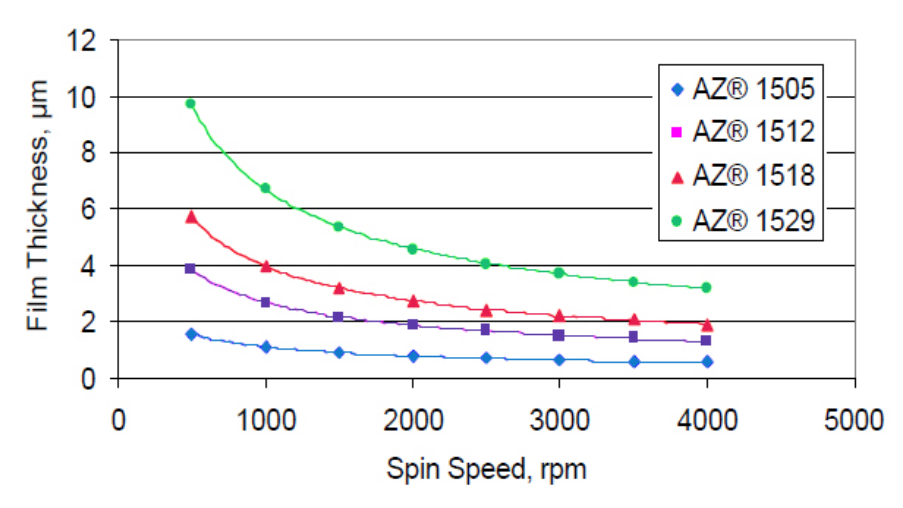
\includegraphics[width=0.7\textwidth]{chap2/az1512-spin-curve.png}
		\caption{Spin curve of AZ-1512HS (Source: EMD Performance Materials\cite{az1500_series_spincurve})}
	\end{figure}
	
	\subsubsection{Skin issues with HMDS}\label{sec:sin_issues}
	When using HMDS and AZ-1512HSHS in conjunction, significant amounts of deposition remenants were found on samples as seen in .%TODO 
	
	\begin{figure}[H]
		\centering
		\begin{subfigure}[b]{0.3\textwidth}
			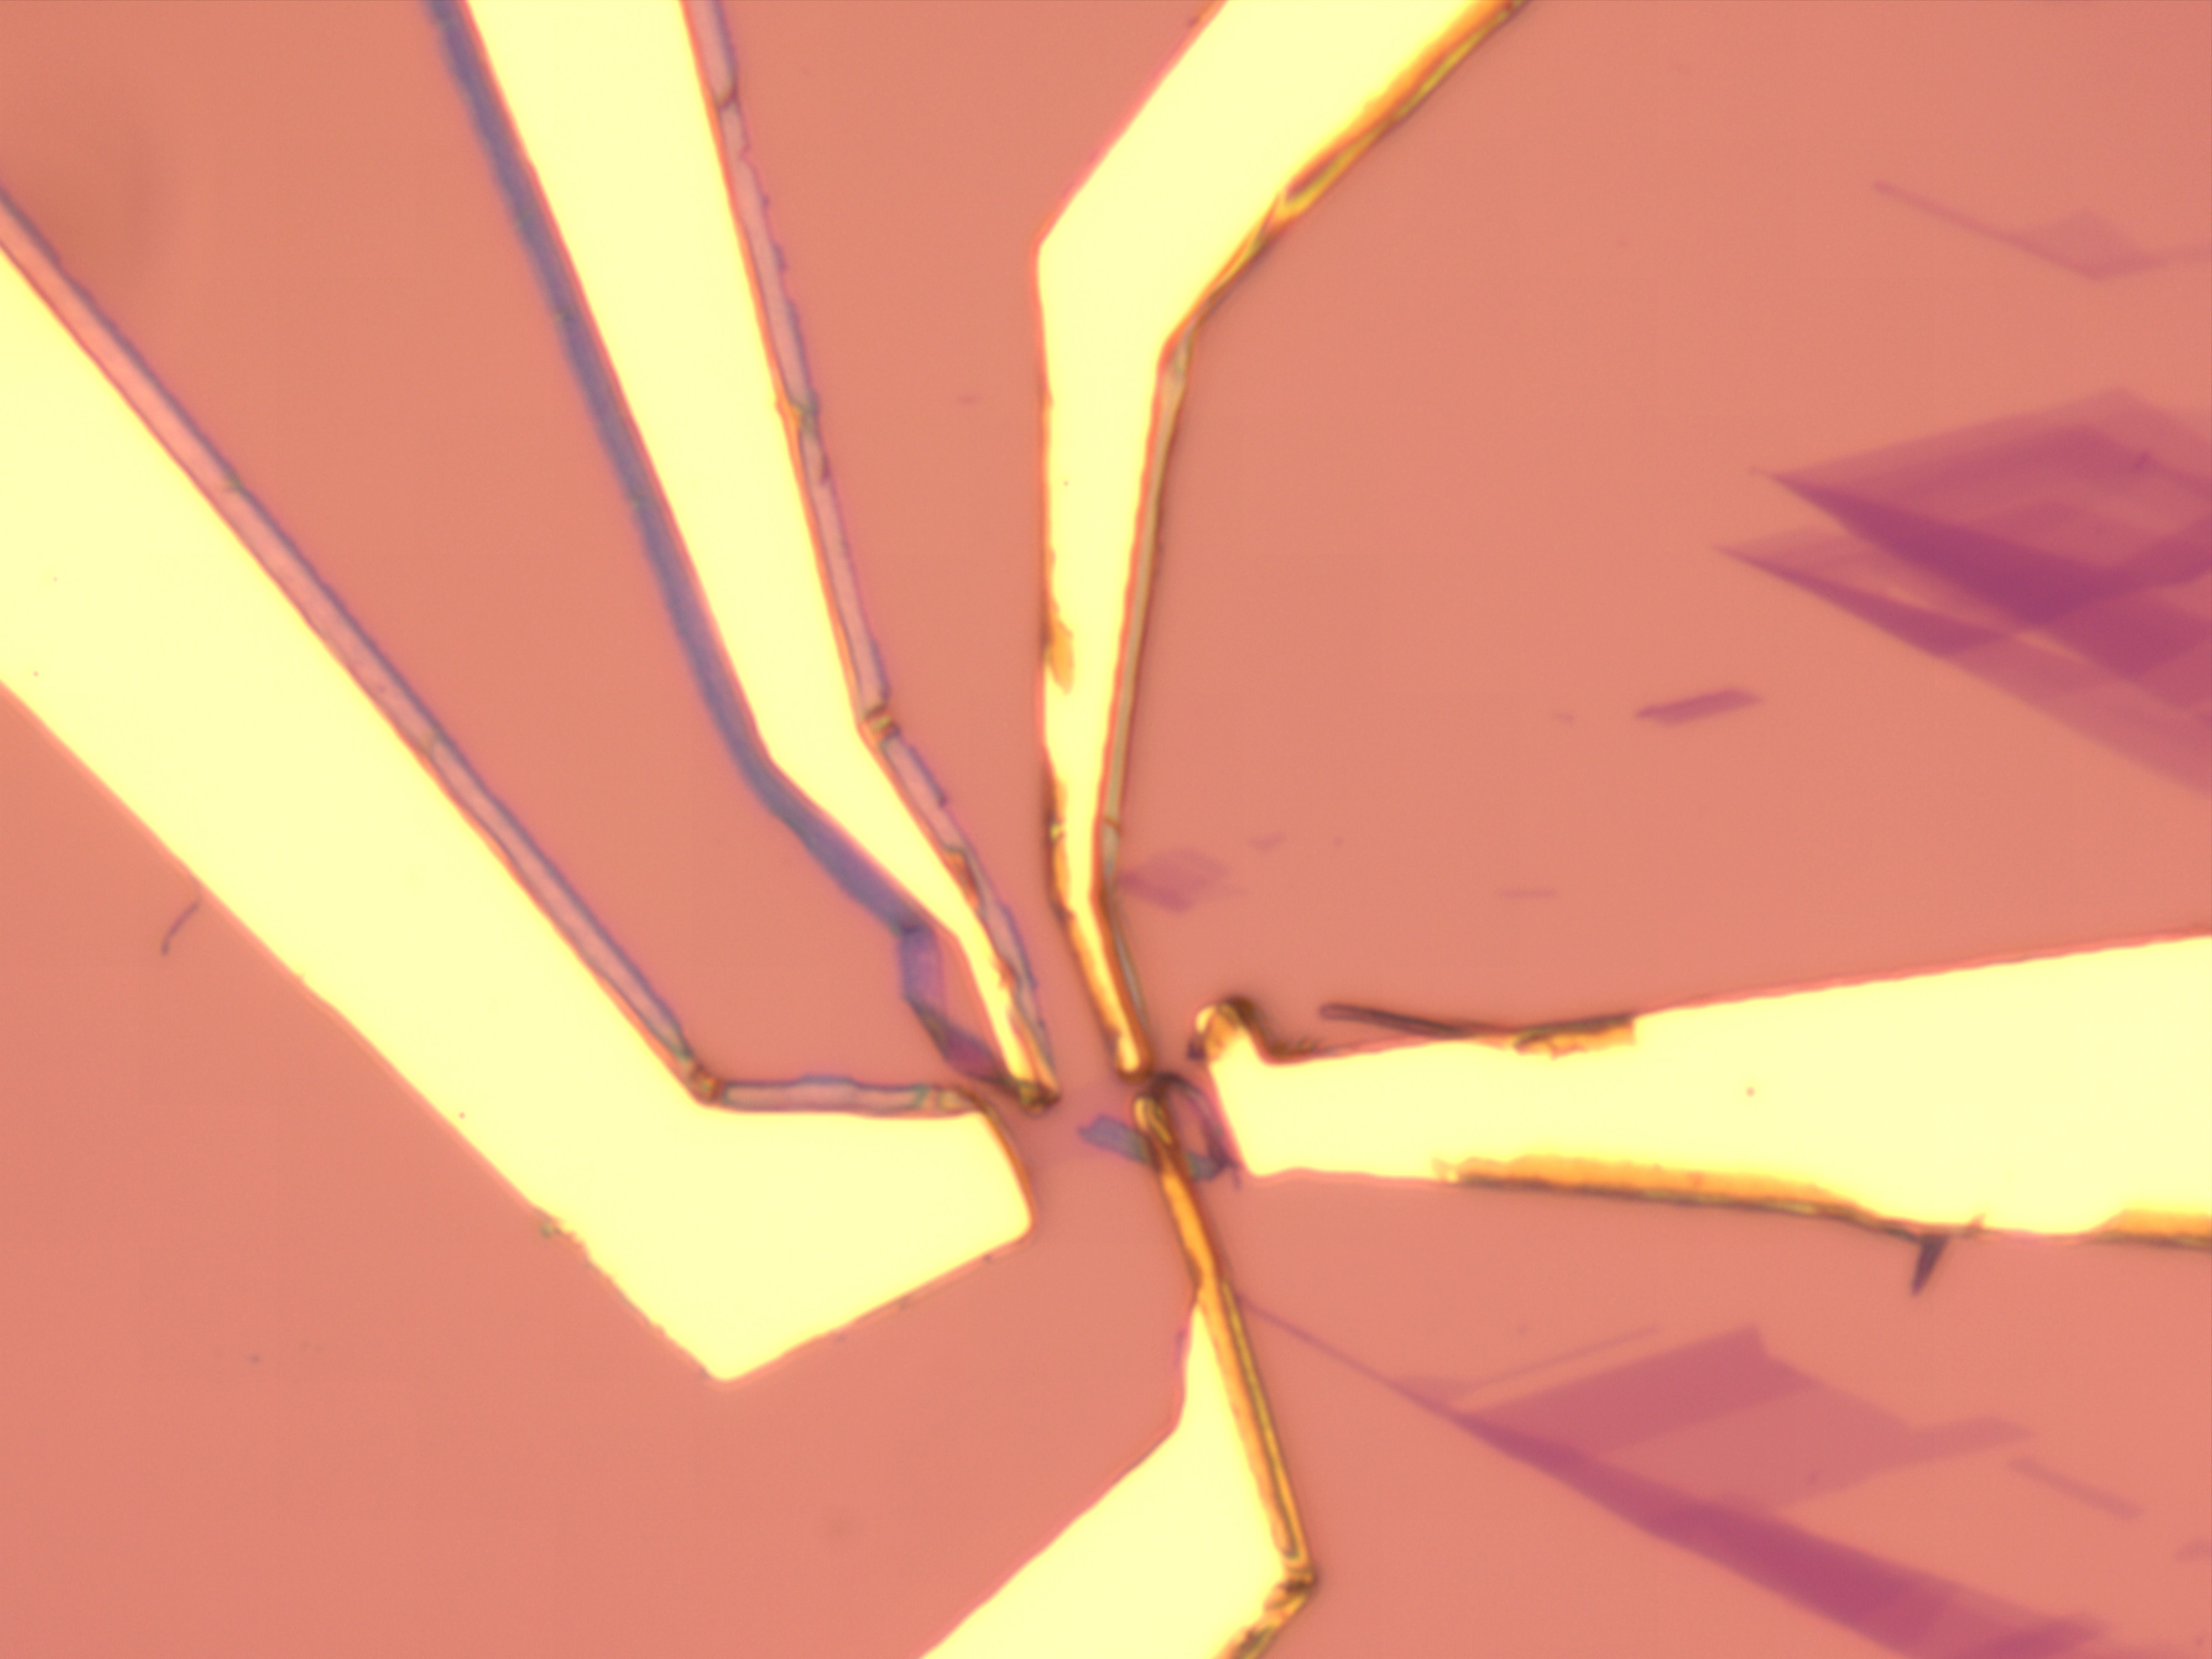
\includegraphics[width=\textwidth]{chap2/skins/Litho01_B07_WA1_F10_100x.jpg}
			\caption{After metal lift off}			
		\end{subfigure}
		\begin{subfigure}[b]{0.3\textwidth}
			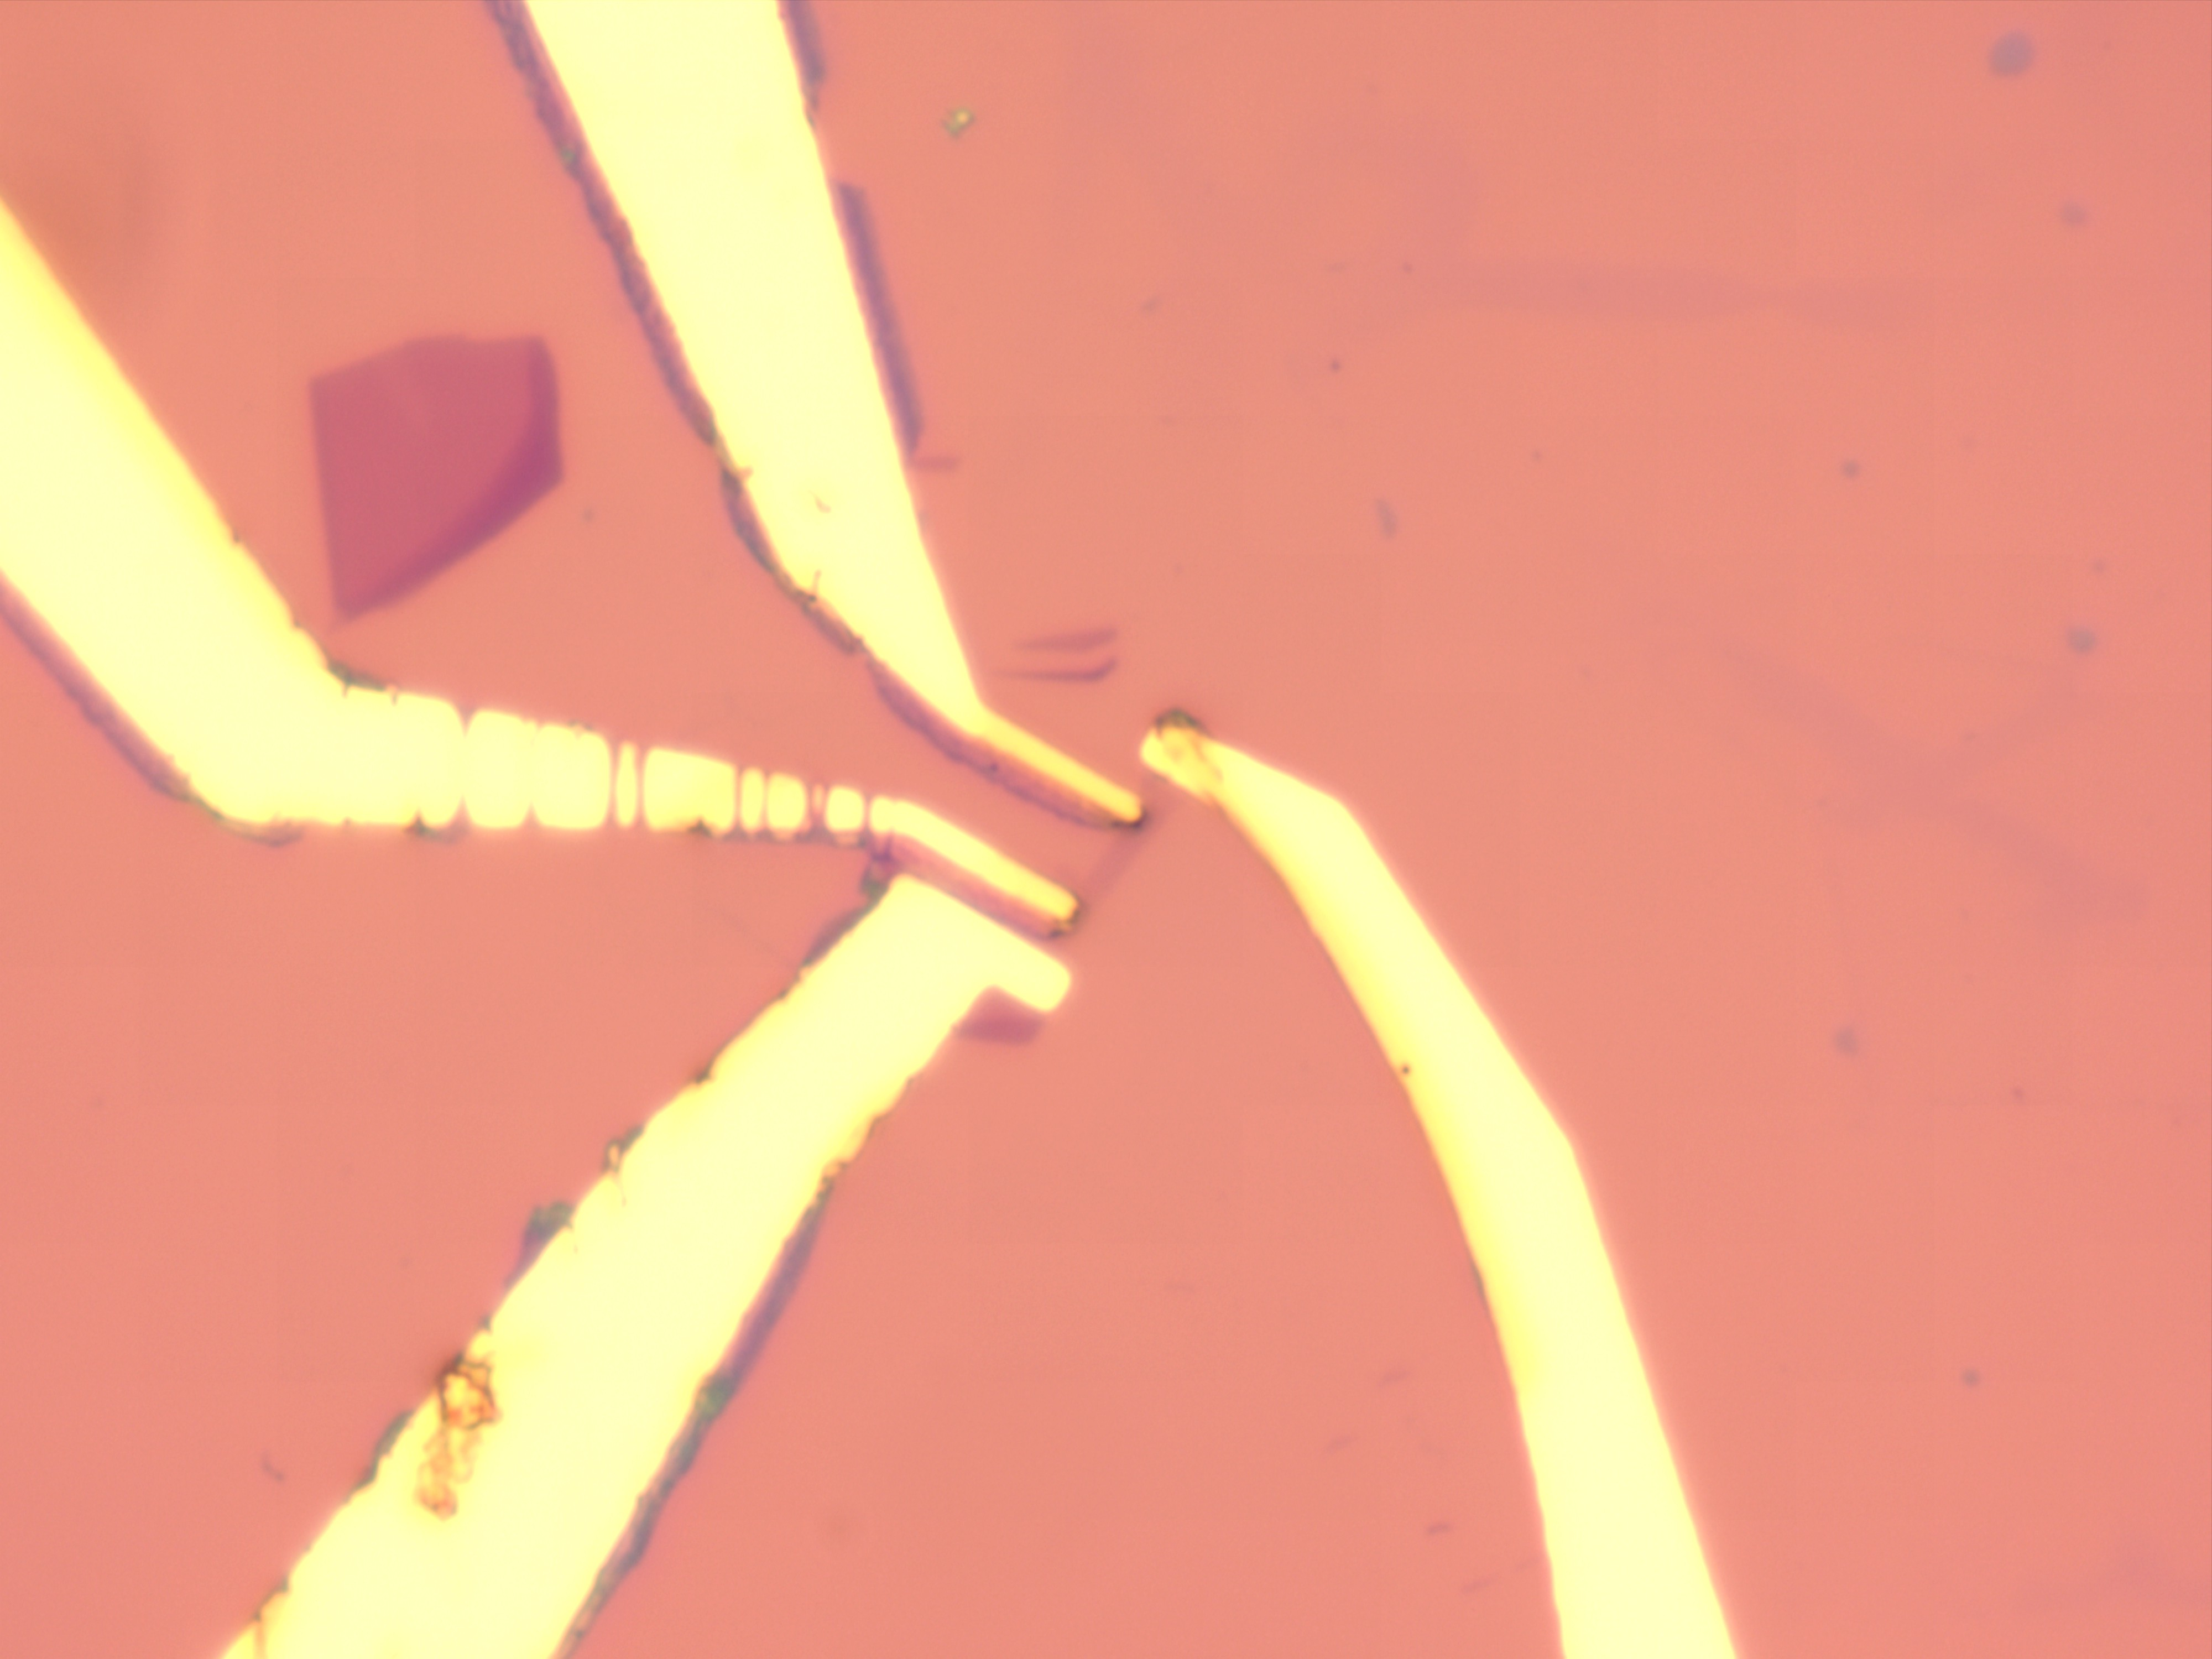
\includegraphics[width=\textwidth]{chap2/skins/1_100x.jpg}
			\subcaption{after 5s ultrasonication}
		\end{subfigure}
		\begin{subfigure}[b]{0.3\textwidth}
			\includegraphics[width=\textwidth]{chap2/skins/2_100x.jpg}
			\subcaption{after 10s ultrasonication}		
		\end{subfigure}
		\caption{Material remanants from lithography}\label{fig:lithography_skins}
		%TODO orientate images.
	\end{figure}
	
	This is likely a result of initial layers of metal deposition (ie, Chromium, see \cref{sec:deposition}) forming layers on the sides of the developed lithography wells, as the skins have very similar geometry to that of either the wells or the edges. Futher evidence that supports this is that the spinning speeds give resist heights (ie, the well edge heights) roughly the same as feature width ($\approx$1$\mu$m minimum).
	
	Sometimes these remenants could be cleaned off, through the use of ultrasonication, however this had a large risk of damaging the graphene, seen in \cref{fig:lithography_skins}.
	
	
	\begin{figure}[H]
		\centering
		\begin{subfigure}[b]{0.3\textwidth}
			\includegraphics[width=\textwidth]{chap2/US/2_100x.jpg}
			\caption{After metal lift off}			
		\end{subfigure}
		\begin{subfigure}[b]{0.3\textwidth}
			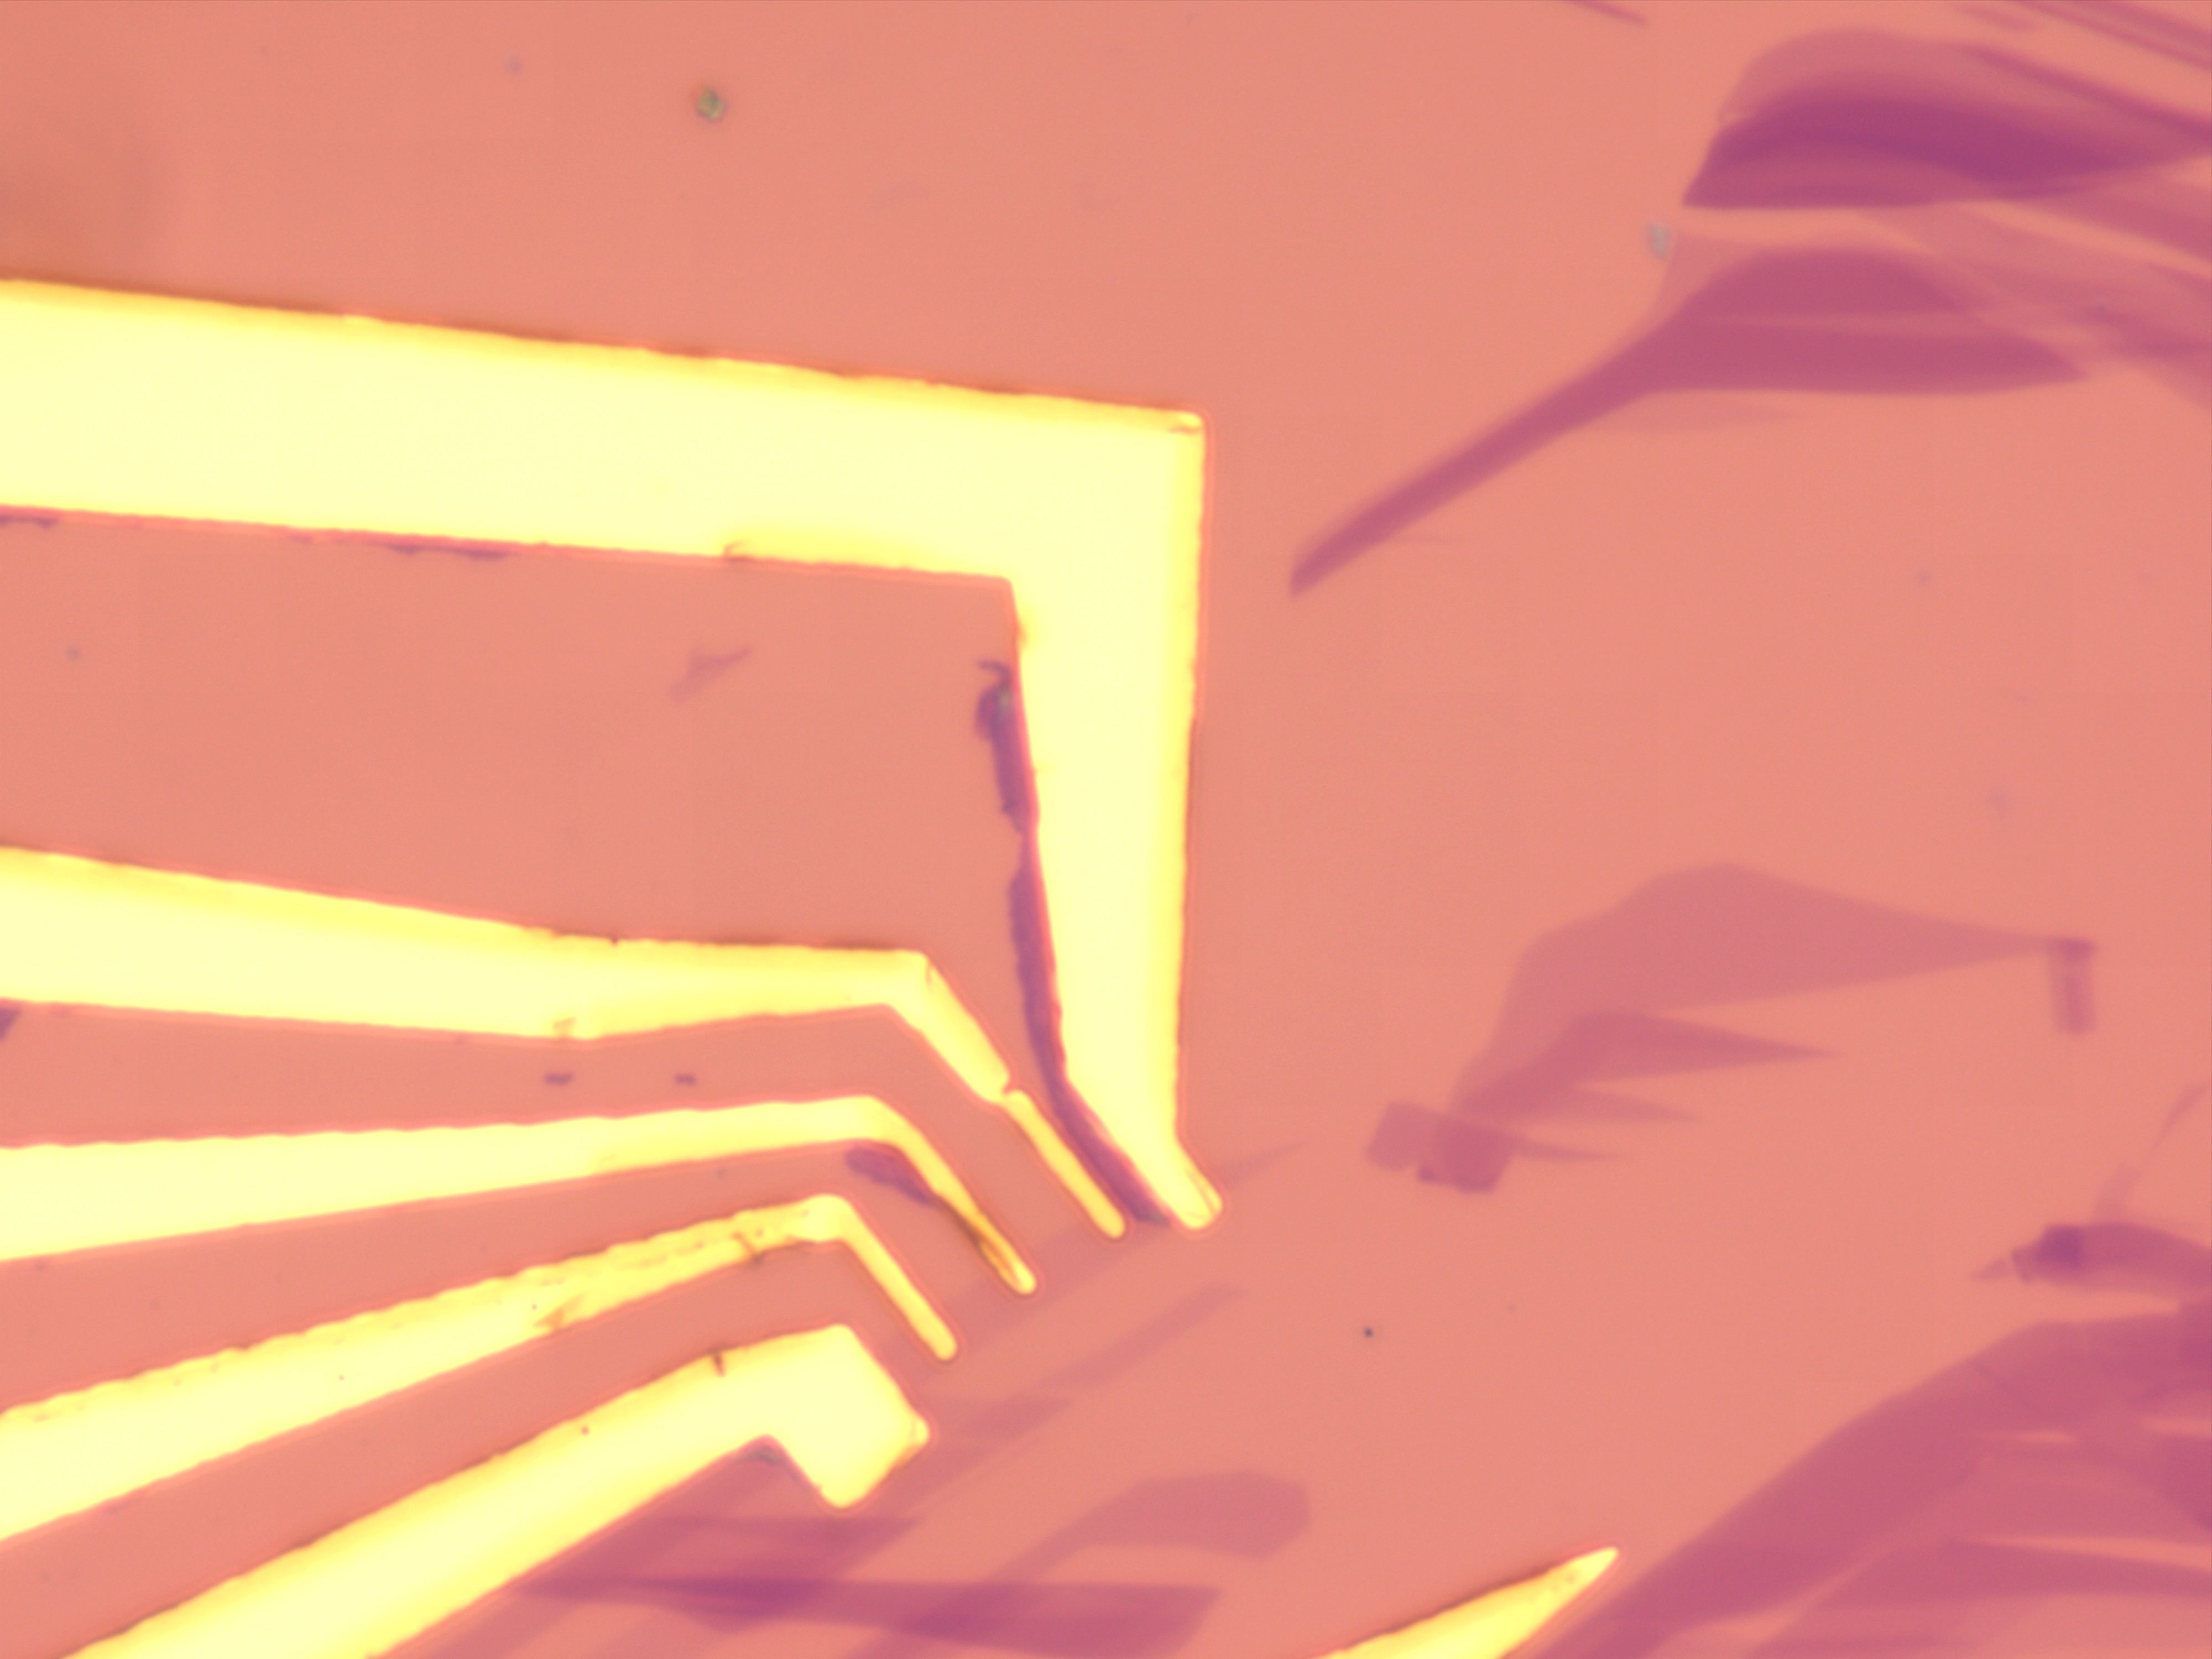
\includegraphics[width=\textwidth]{chap2/US/2_100x_after6sAcetoneUS.jpg}
			\subcaption{after 5s ultrasonication}
		\end{subfigure}
		\begin{subfigure}[b]{0.3\textwidth}
			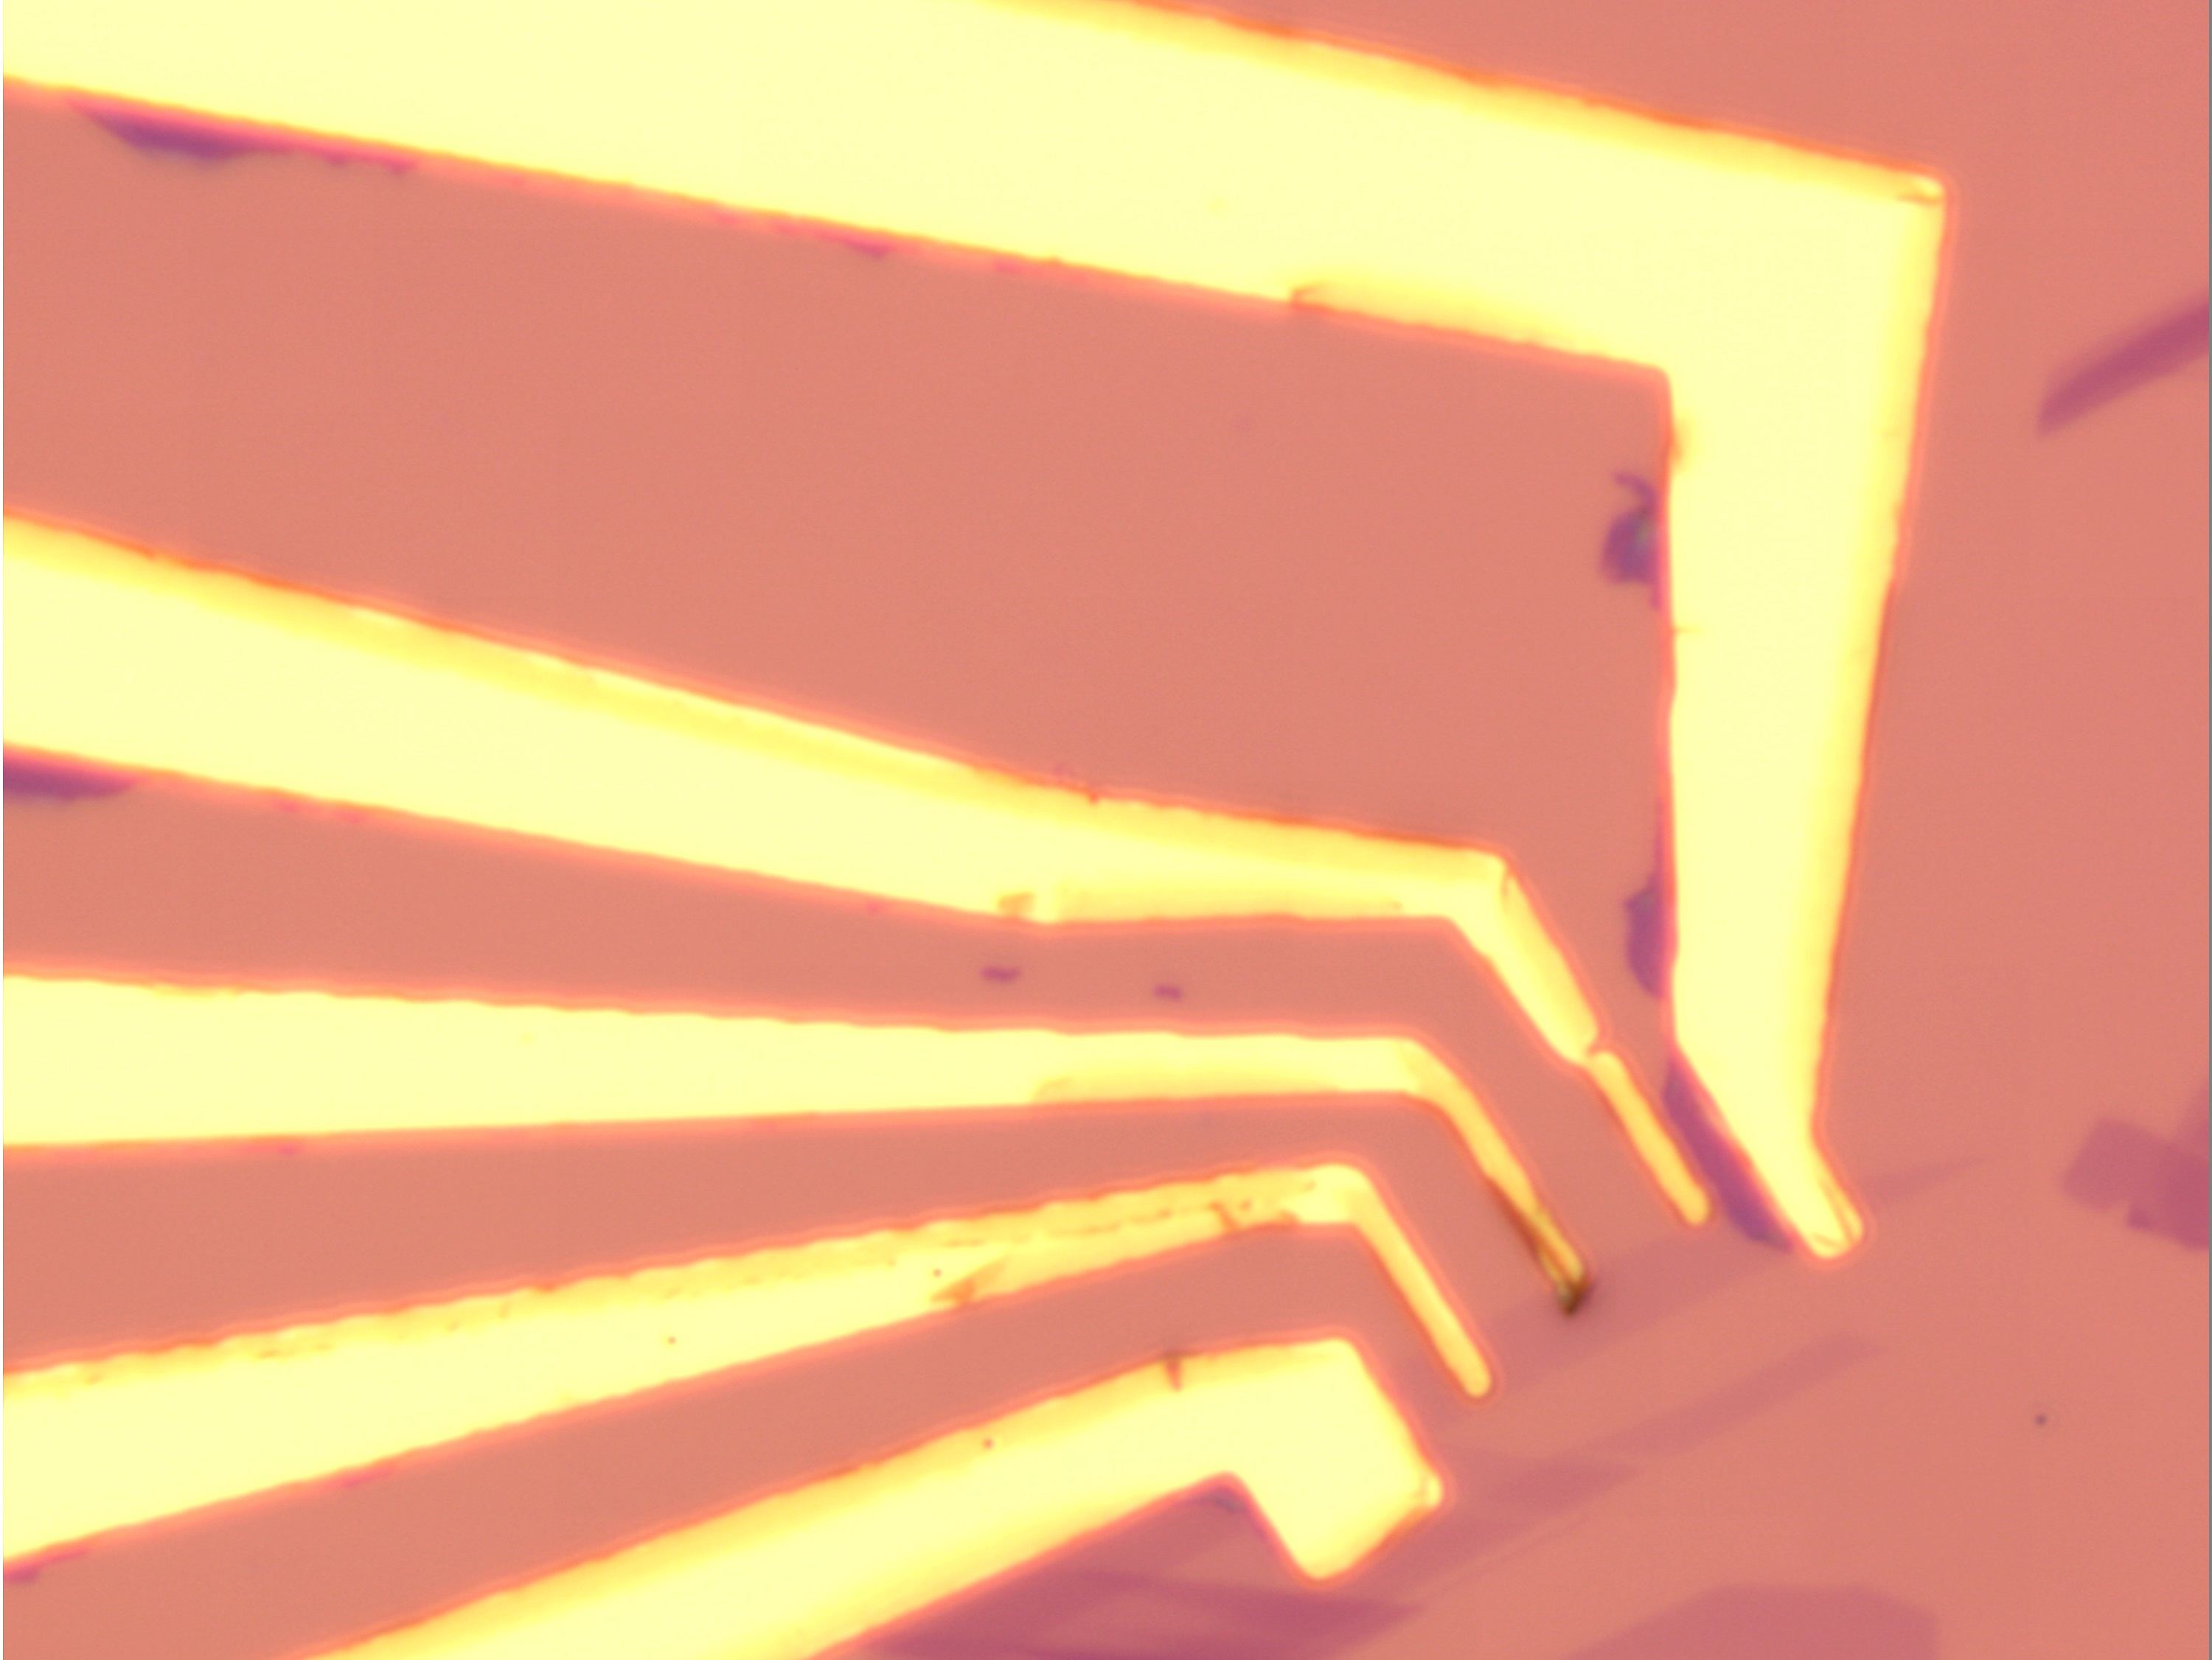
\includegraphics[width=\textwidth]{chap2/US/2_100x_after10sAcetoneUS.jpg}
			\subcaption{after 10s ultrasonication}		
		\end{subfigure}
		\caption{Material remanants from lithography}\label{fig:lithography_skins_us}
		%TODO orientate images.
	\end{figure}
	
	\subsubsection{LOR-1A \& AZ-1512HS}
	An issue with a single layer photoresist processes is that well edges allow deposited materials to adhere, leaving 'skins'. One way to prevent this from happening is to use a multilayer process. Two resist layers are spun onto the sample, with the bottom film being more sensitive to the lithography process than the top (ie, develops faster, or is more sensitive to exposure). When developed, the bottom layer \textit{undercuts} the top layer, stopping adhesion the to edges of the well when material is deposited. This process id depicted in \cref{fig:bilayer_lithography}.
	
	\begin{figure}[H]
		\centering
		
\includegraphics[width=0.3\textwidth]{placeholder}
		\caption{Bilayer lithography process}\label{fig:bilayer_lithography}
	\end{figure}
	
	Rather than a photoresist, LOR-1A is a lift off resist. When the films are exposed to the developer, LOR-1A is also lifted off with the soluble AZ-1512HS. Additional material is pulled and dissolved from the well, leaving the desired undercut effect. %TODO CHECK HOW IT REALLY WORKS.
	
	\subsection{Exposure}\label{sec:exposure}
		After spinning, a mask writer tool is used to expose the wafer and resist films to UV light to develop desired pads. A mask writer usually is composed of a DMA (Digital Mirror Array) which allows filtering to pixel like squares. %TODO CHECK DMA
		
		An important parameter played with in this process is the exposure time, which affects your ability to develop fine structures. By using an array of different exposure times (\cref{fig:exposure_array}), we were able to optimise our feature exposure for a typical developing time.
		
	\begin{figure}[H]
		\centering
		
\includegraphics[width=0.3\textwidth]{placeholder}
		\caption{Developing an exposure array on \silicondioxide}\label{fig:exposure_array}
	\end{figure}
	
	Prepared CAD files, that specify the structure for desired contact pads onto devices, are used by the DMA to iteratevly expose small areas of the film. These exposed areas undergo a chemical change, changing the structural properties for development.
	
	\subsection{Developers}\label{sec:developer}
	Developers are used to dissolve exposed / unexposed areas of photoresist films. For example, we use AZ-726 in conjunction with AZ-1512HS. Setting a development time complementary to your exposure time is important to not overdevelop your features, as material in prodximity to exposed areas is at risk of structural damage.
	
	
	\section{UV Ozone surface preparation}\label{sec:uv_ozone}
	
	\section{Deposition}\label{sec:deposition}
	
	\subsection{Oxide}
	
	\section{Lift-off}\label{}
	\subsection{Ultrasonication}
	
	\section{Oxide transfer}
	\subsection{Printing}
	\subsubsection{Al$_2$O$_3$}
	\subsubsection{SnO}
	\subsubsection{Bi$_2$O$_3$}
	
	\subsection{Smearing}
	\subsubsection{Ga$_2$O$_3$}
	
\end{document}